\documentclass{article}
\usepackage[utf8]{inputenc}
\usepackage[round]{natbib}
\usepackage{amsthm}
\usepackage{amssymb}
\usepackage{float}
\usepackage{tabularx}
\usepackage[toc,page]{appendix}
\usepackage{cleveref}
\usepackage{graphicx}
\usepackage{enumitem}
\usepackage{tikz} % To generate the plot from csv
\usepackage{pgfplots}
\theoremstyle{definition}
\newtheorem{ftsdef}{Definition}
\newcolumntype{R}{>{\raggedleft\arraybackslash}l}%

\title{Dissertation}
\author{Michael Gallagher}

\begin{document}

\maketitle

%\listoffigures

%\listoftables

\tableofcontents

\section{Introduction}
TODO this.

The aim of this project is to explore the applicability of fuzzy logic to time series analysis. This paper examines and compares various fuzzy time series models proposed in the literature.

The debate over the usefulness of technical analysis is still up in the air. There are many studies demonstrating excess returns compared to a uninformed strategies such as buy and hold, even after transaction costs. As shown in the literature review, many aspects and techniques of technical analysis have been studied including visual patterns such as ``Head \& Shoulders'', trend lines, moving averages, Japanese Candlestick Charting and neural networks. Many explanations justifying technical analysis have been proposed including market psychology, market inefficiencies and insider trading. The more recent studies have used well regarded statistical techniques, out of sample verification, parameter optimisation and transaction costs.

The perception of technical analysis among experts varies significantly. The empirical nature of technical analysis makes conclusive evaluation difficult. Data snooping, where different combinations of variables are combined until a model that matches the data is found, is a concern in many studies. The issue is that in a study of 100 random technical patterns, 5 of them will generate statistically significant excess returns. This risk can be reduced by testing the trading strategy against a sample set of data, but the question can linger as to why one technical trading strategy is more effective than another and why is it effective on some sample data but not all. The studies that demonstrate insignificant returns or losses may have been tested against a dataset to which technical analysis doesn't apply, or on the contrary, strategies that demonstrated profit such as a moving average cross may have been tested in a time when the market featured significant trends which the moving average indicator is suited to.

This paper takes a different approach to performing technical analysis. Many studies have been carried out on technical trading strategies that are actively used in the financial industry. Often these strategies have been in use for several decades, discovered out of empirical observation of visual data at a time before it was possible to verify the techniques computationally. However, the market conditions and behaviour may have changed since the discovery of these techniques. Newer markets may have characteristics not reflected by traditional technical analysis. 

The model proposed in this paper aims to derive these characteristics by examining the historical price data of a security using fuzzy time series analysis and identifying statistically significant regularities. 

Fuzzy time series analysis identifies fuzzy relationships between points on a time series and uses these to forecast observations. A time series is a sequence of real numbers that change over time, a graph of price being an example. Fuzzy time series models examine a history of data and the change in price between one point in time and the next. These fluctuations are seen as relationships between those points in time. Fuzzy time series analysis supposes that fluctuations at certain points are likely to happen again, and that relationships obtained when examining past data can be used to predict changes.

\section{Literature Review}

\subsection{Emperical Analysis}

\begin{figure}[H]
    \centering
    \includegraphics[width=0.8\textwidth]{images/blackwhite.png}
    \caption{Moving-Average Cross Indicator}
\end{figure}

Technical analysis is a form of financial analysis where past price behaviour is used to forecast future price in financial markets. It is one of several methods of analysing financial securities. Other methods include fundamental analysis, which involves analysing the health of a security by viewing information such as company earnings, and sentiment analysis, performing analysis on written text or speech regarding a financial security or market and extracting the sentiment of the author or the market towards it \citep[p. 2]{ahmad2011affective}.

\cite{foundations} argued that ``the general goal of technical analysis is to identify regularities in the time series of prices by extracting non-linear patterns from noisy data''. Examples of this form of analysis include identifying trends in a graph of price movement, or concluding that a price is unlikely to go lower than the 52-week low. Specific techniques are discussed in \Cref{app:tatechniques}.

\subsubsection{History}

The use of this form of analysis has been documented for several hundred years. One of the first uses of technical analysis dates back to Japan in the 18th Century. In 1710 Japan's rice market had matured enough to begin use rice coupons instead of trading physical rice. Their receipts were traded constituting the first Futures trades ever recorded \citep[p.15]{jcct1991}. 

Munehisa Homma was a rice merchant in Japan, who amassed great wealth trading these rice coupons and is sometimes credited as the Father of Japanese Candlestick Charting. Although it is unclear whether Homma actually used Japanese Candlestick Charting techniques, it is recorded that he used the history of price movement to gauge the emotions of the market at the time, ``When all are bearish, there is cause for prices to rise. When everyone is bullish, there is cause for the price to fall''. Following Homma different charting techniques were introduced, until the introduction and popularisation of Japanese Candlestick Charting for technical analysis in the mid 19th Century \citep[p.18]{jcct1994}.

In the west, Dow Theory was developed and expanded on in the early 20th Century, leading to works \citep{edwards2012technical} that directly influence technical analysis today.

Even with such a diverse history the use of technical analysis is still a hotly debated topic. Experts and Academics are divided in its use \citep{foundations}, the influential \textit{A Random Walk down Wall Street} concluding it is as valid as Alchemy when put under scientific scrutiny \cite[p.159]{randomwalk2012}. Nonetheless, it appears a significant number of analysts incorporate technical analysis, with a study by \cite{examininguse1997} finding a mean importance of 35\% was given to technical analysis by respondents in various investment banks, and \cite{cheung2000currency} characterising 30\% of Foreign-Exchange traders as Technical Traders. 

\subsubsection{Performance of technical analysis}

\cite{taprofitability} performed a comprehensive review of 95 studies of technical trading strategies from between 1988 and 2004. Although there is a significant number of studies before this date, they note that prior to \cite{lukac1988} studies suffered from a number of problems, which \cite{brock1992} summarises as:

\begin{enumerate}[label=\roman*]
\item Relatively short time periods being examined 
\item Studies generally not computing significance levels 
\item Studies are both designed and tested on the same data
\end{enumerate}

In mitigation \cite{taprofitability} argue that modern studies ``typically
increase the number of trading systems tested, assess risks of trading rules,
perform statistical tests with either conventional statistical tests or more sophisticated bootstrap methods, or both, and conduct parameter optimization and out-of-sample verification''.

\cite{taprofitability} found that of these modern studies, 56 found positive results, 20 obtained negative results and 19 indicated mixed results. 

They offered several theoretical explanations for the positive results. Econometric models such as the noisy rational expectations model postulate that the current price does not reveal all information about a security because of noise, and the market shows a systematic slowness in adjusting to new market information, which can be exploited with technical analysis. Behavioural models propose that price is affected by market psychology which can be predicted using technical analysis, akin to the original uses of Technical Analysis. Technical analysis charting methods may also be equivalent to non-linear forecasting methods in chaos theory.

They also offered empirical explanations for the results, such as trends in price before news such as central bank interventions, and order flows where the take profit and stop loss of orders clustering around round numbers. Other empirical explanations offer the possibility of false positive trading profits. Temporary market inefficiencies may occur, where new trading strategies offer short term gains before they become more widely used and cease to offer an advantage. Also market microstructure deficiencies where studies do not adequately take transaction costs and other market factors into account may result in inaccurate results. 

\cite{taprofitability} acknowledge that despite the positive evidence and improved procedures, many academics and professional analysts are sceptical about technical analysis and technical trading strategies. They point to \cite{assetpricing} who says that ``trading rules that reliably survive transactions costs and do not implicitly expose the investor to risk have not yet been reliably demonstrated''. They interpret this to mean that the scepticism is due to data snooping problems, where trading strategies over-fit the testing data, and insignificant profits after taking adjustments for transaction costs and risk.

In the professional world, it could be due to the difficulty in experimentally verifying some technical analysis techniques, many of which rely on visual cues in the eyes of an Expert. The existence of a pattern is subjective. Experts looking at the same data may see different, sometimes contradictory patterns, fuelling a controversy that technical analysis is nothing more than pseudo-analysis. Also with most studies finding some technical trading strategies successful and many unsuccessful, it might be perceived as safer to ignore technical analysis altogether.

\subsubsection{Econometric Time Series Analysis}

``I believe there is no other proposition in economics which has more solid empirical evidence supporting it than the Efficient Market Hypothesis'' stated \cite{jensen1978some}. The Efficient Market Hypothesis claims that the price of a security is extremely efficient at reflecting most of the information about that security. When news is public the market will very efficiently arrive at a price for the security that reflects the impact of the news. This claim has major consequences; that both technical analysis and fundamental analysis are unable to help an investor achieve a greater profit than if a random selection of securities were invested in \citep{emhAndCritics}. 

While there is still a lot of support for this model, strict adherence to it does not offer the complete picture. If the markets were perfectly efficient then the price would simply jump between points as individual news was released. In reality there is a large amount of noise, volatility and uncertainty in the market. Very often it is not clear what impact some news should have. And of course the accuracy of market information and the availability of the information to the public add further uncertainty to the price movement. 

\cite{malkiel1970efficient} argue that these issues do not necessarily imply an inefficient market unless there are investors who can consistently make better evaluations of available information. They argue that the hypothesis that the price of a security ``fully reflects'' all available information at any point in time is an extreme null hypothesis, which we do not expect to be literally true. Different efficient market models have been proposed with characteristics that can be evaluated separately, allowing researchers to pinpoint where the hypothesis breaks down. The \textit{weak form} model claims that price reflects all past publicly available information. The \textit{semi-strong form} model claims that the price reflects all past publicly available information and also that price will instantly change as new information is made available. The \textit{strong form} claims that price reflects all public and non-public information.

The Random Walk Hypothesis says proposes that the price of a security represents a 'random walk' around its intrinsic value, and consequently that price movements can not be predicted. \cite{malkiel1970efficient} describes the random walk model as a ``fair game'' model in which the conditions of market equilibrium can be stated in terms of expected returns, but note that an efficient market does not require a random walk. 

\cite{lo1988} studied weekly by comparing variance estimators of stock market returns. They argue that if prices are generated by a random walk, then the variance of the monthly sample log-price, i.e.\ the variance of the log of the difference in monthly price, must be 4 times as large as the variance of the weekly sample. Their findings strongly reject the random walk hypothesis, but are careful to note that ``this rejection does not necessarily imply the inefficiency of stock-price formulation''.

Almost 30 years ago, \cite{indefenseof} showed that past prices combined with other information, such as non-public information, can achieve unusual profit. They claim that non-price information creates opportunity that can be efficiently exploited using technical analysis. As non-public information is revealed to an investor, it is unclear as to the extent that this information has been revealed. If the investor knows the behaviour that a market would demonstrate if this information was widely distributed, he or she could examine the past price movements and determine a probability that the information has been revealed, and thus determine if there is still opportunity for a profitable investment.

While this demonstrates a use for past price data, it only demonstrates use when combined with other valuable information, and thus does not contradict the Efficient Market Hypothesis which only states that attempting to make profits by exploiting currently available information is futile \citep{taprofitability}.

\subsubsection{Human Perception}

Although the evidence supporting technical analysis is inconclusive, it is still regarded as an important forecasting tool by many analysts. One of several explanations by \cite[p.45-71]{aronson2011evidence} is that humans suffer cognitive biases when determining the significance of visual patterns in their analysis. Many experts believe they can spot visual patterns such as price trends on a graph, and would take the claim that these trends are irrelevant as ridiculous. However when developing or practising a trading system based on patterns, technical analysts can succumb to confirmation bias by giving a higher significance to evidence that supports the pattern they're looking for as opposed to evidence for other patterns that might be available. Also when determining the efficacy of these systems based on past data, hindsight bias can lead to certain patterns appearing obvious after their formation. This leads an expert to think this pattern is easily detectable, even though while the pattern was forming the evidence for that particular pattern was indecisive, and possibly pointed to other, contradictory patterns \cite[p.62]{aronson2011evidence}.

Another explanation is that technical analysis appeals to behavioural psychology. If a large amount of investors are searching for similar patterns, then the outcome following these patterns may become a self-fulfilling prophecy. A study by \cite{examininguse1997} finds that 49\% of Foreign-Exchange Technical Analysts explicitly cite this as a reason. These points are disputed by Malkiel however, stating "The problem is that once such a regularity is known to market participants, people will act in a way that prevents it from happening in the future" \cite[p.162]{randomwalk2012}.

\subsection{Fuzzy Set Theory}

\subsection{Fuzzy Time Series}

\cite{box2013time} describes a time series as ``a sequence of observations taken sequentially in time''. A core feature of a time series is that typically adjacent observations are dependent, such that the value of the observation at time $t$ is somewhat dependent on the value at time $t-1$. The practical implications of this feature is that through time series analysis it is possible to model a time series and use this model to forecast observations.

A fuzzy time series is a model of a time series that uses fuzzy set theory to find relationships between points on the time series and use these relationships to forecast observations. According to \cite{chen1996forecasting}, "the main difference between a a fuzzy time series and conventional time series is that the values of the former are fuzzy sets and the latter are real numbers".

The typical use of a fuzzy time series is to forecast observations on the time series using historical data. Studies using fuzzy time series have been carried out on forecasting university enrolment \citep{song1993forecasting, song1994forecasting, chen1996forecasting, tsai2000forecasting, chen2004new, cheng2006trend, lee2006pattern, huarng2006ratio, tsaur2012fuzzy}, Stock Market price \citep{huarng2005type, cheng2006trend, lee2006pattern, huarng2006ratio, Chen2007fib, chu2009fuzzy}, Foreign-Exchange rates \citep{tsaur2012fuzzy}, population change \citep{tsai1999study} and temperature \citep{temperatureprediction2000, lee2006pattern}. 

\subsubsection{Basic Model}
\label{basic}
\cite{song1993forecasting} pioneered the fuzzy time series model providing the definitions for the concept and a method for modelling a time invariant fuzzy time series. The method was shown to be better than the Linear Regression Method for forecasting student enrolments at the University of Alabama. Their model fuzzified points on the time series into fuzzy sets and defined fuzzy relations between these sets. They use an arithmetic defuzzification algorithm to interpret the results and claim ``it is not difficult to jump to the conclusion that in the interpretation of the output results, experience knowledge is still needed''.
 
\cite{chen1996forecasting} made improvements this model by using simplified mathematical operations instead of computationally expensive max-min composition for defining fuzzy relations. This method, while being more efficient, was also shown to be more accurate than the method proposed by \cite{song1993forecasting}. Many future studies follow the proposed method, changing some individual steps in order to improve accuracy. To aid explanation of future studies, the proposed algorithm is summarised as follows:

\begin{description}
\item[Step 1] Define a universe of discourse over the maximum and minimum values of observations on the time series and partition it into several intervals
\item[Step 2] Define fuzzy sets on the universe of discourse. These fuzzy sets are composed of each of the defined intervals and their membership in that fuzzy set. Fuzzify the time series into these fuzzy sets
\item[Step 3] Calculate the maximum membership of the fuzzified data and form fuzzy logical relationships between the fuzzy values of neighbouring observations on the time series
\item[Step 4] Group the fuzzy logical relationships into groups such that relationships defined as $R(t,t-1)$ have the same fuzzy value for $t-1$. That is, the relationships have the same fuzzy value on the left-hand side. These groups are called fuzzy logical relationship groups
\item[Step 5] Forecast observations. Let the fuzzy value of $F(t)$ be $A_i$. This step is concerned with forecasting the fuzzy value of $F(t+1)$
\begin{enumerate}
\item If  $A_i \rightarrow A_k$ is the only fuzzy logical relationship in the fuzzy logical relationship group associated with $A_t$, then $F(t+1)$ is forecast as $A_k$ 
\item If there are multiple fuzzy logical relationships associated with $A_i$, such that with fuzzy logical relationship group $A_i \rightarrow A_{i}, A_{j}, \ldots, A_{k}$, then $F(t+1)$ is forecast as $A_{i}, A_{j}, \ldots, A_{k}$
\item If there are no fuzzy logical relationships associated with $A_i$, then $F(t+1)$ is forecast as $A_i$
\end{enumerate}
\item[Step 6] Defuzzify the forecast fuzzy set using the Centroid method. Practically, this involves calculating the average of the midpoints of each interval which has a maximum membership in a fuzzy set that is forecast for $F(t+1)$
\end{description}

\subsubsection{Higher-Order Models}

A first-order time series is described in \Cref{basic}. Fuzzy relations are defined between each adjacent point and only the most recent value in a time series is used for forecasting.

An $n$th-order or higher-order fuzzy time series is one where where there is a simultaneous relationship between multiple points on the time series, not just adjacent observations. There are fuzzy logical relationship groups defined between all points $1,2,\ldots,n$ spaces in time apart. The most recent $1,2,\ldots,n$ observations are used to forecast fuzzy values, which are then composed and defuzzified.

\cite{tsai1999study} found that a second-order fuzzy time series lead to more accurate predictions when forecasting population, particularly when the number of intervals on the fuzzy time series was increased. \cite{tsai2000forecasting} compared the performance of 5 higher-order time series models on predicting university enrolments, and found the higher-order models to be more accurate, with the model increasing in accuracy with every increase in the order of the time series, up to a fifth-order time series.

\subsubsection{Interval Selection}

Deciding on the size and number of interval partitions on the universe of discourse is an important issue \citep{Huarng2001effective,  huarng2006ratio}. If there are too few intervals, there will be fewer fluctuations in the fuzzy time series \citep{Huarng2001effective}, which results in less precise fuzzy logical relationships. More intervals also result in each fuzzy value representing a small range of values, which result in a more accurate crisp value during defuzzification. However, too many intervals will not be recognised by an expert which negates some of the benefits of using fuzzy logic.

Many studies use the same, arbitrarily selected interval size such as $1000$ \citep{song1993forecasting, song1994forecasting, chen1996forecasting, tsai2000forecasting, chen2004new}. However, several studies have demonstrated that using more intervals can improve accuracy. \citep{tsai2000forecasting} shows that when modelling a higher-order fuzzy time series, increasing the number of intervals dramatically improved results. They found that by increasing the number of intervals from $7$ to $19$, the root mean square error of the forecast results fell from $609.22$ to $199.32$. \cite{tsai1999study} also found a similar improvement when increasing the number of intervals, for both first-order and higher-order time series. \cite{chen2004new} proposed a method for forecasting university enrolments which used 13 intervals instead of the usual 7, and an extra step which further divided each interval into 4 parts in order to detect a trend of movement. Although this can not be attributed solely to increasing the number of intervals, it also demonstrated significantly improved forecasting accuracy. 	

\cite{Huarng2001effective} empirically study how the length of intervals affects the forecasting results of a fuzzy time series. They examine two approaches, distribution- and average-based interval length. Both of these approaches are derived using the absolute difference of any two consecutive observations, and ensure that at least half of these differences in the time series are reflected by the intervals. 

Both methods utilise a mapping table to approximate the base of the interval based on the average first difference. The distribution-based approach plots the distribution of the first differences using an interval that is derived from the mapping table. The interval on the distribution containing the largest first difference that is at smaller than at least half the distributions is chosen as the interval for the fuzzy time series. The average-based approach involves deriving the base from the mapping table, calculating half of the average first difference, rounding this value to the derived base and using this value as the interval.

\cite{Huarng2001effective} found that these approaches improved the accuracy over the arbitrarily selected interval used in prior studies, with the average-based approach performing better than the distributions based approach. They compared the results of these approaches with 9 arbitrarily chosen but small interval lengths, and found that the average-based approach resulted in the best and second best predictions for university enrolments and the Taiwan Stock Exchange Weighted Index (TAIEX) respectively. They also found that smaller interval lengths did not always result in a more accurate prediction.

\cite{huarng2006ratio} explored using the ratios between the absolute differences to define intervals. The rationale behind using ratios to determine intervals was that the momentum of the time series oscillates more or less depending on the context. The same source of data, such as a stock price, may have different optimal interval lengths depending on the amount of activity of the time series at that time. Using interval lengths that reflect the relative difference between observations takes this into account without using a secondary data source such as volume.

\cite{huarng2006ratio} compared the approach to the average- and distribution-based approaches as well as several arbitrarily chosen similarly sized intervals. The ratio based approach resulted in the best accuracy for the methods tested when forecasting university enrolment, TAIEX price and inventory stock. They also found that the optimal interval length changed between data sets from the same data source, and that the ratio based approach was effective at approximating the optimal length.

\section{Design}

\subsection{Fuzzy Time Series}
\label{fts-design}
The following definitions describe a general model of a fuzzy time series.

\begin{ftsdef}
\label{def1}
Let $Y(t)(t= \ldots,0,1,2, \ldots)$, a subset of $\mathbb{R}$, be the universe of discourse on which fuzzy sets $f_i(t)(i=1,2,\ldots)$ are defined and let $F(t)$ be a set of $f_i(t)(i=1,2,\ldots)$. Then $F(t)$ is a fuzzy time series on $Y(t)(t= \ldots,0,1,2, \ldots)$.
\end{ftsdef}

\begin{ftsdef}
\label{def2}
Suppose $F(t)$ is caused by $F(t-1)$ only, then this fuzzy relation can be expressed as $F(t)=F(t-1) \circ R(t,t-1)$, where $R(t,t-1)$ is the fuzzy relationship between $F(t-1)$ and $F(t)$. The model $F(t)=F(t-1) \circ R(t,t-1)$ is called the first order model $F(t)$, where $F(t-1) \rightarrow F(t)$ denotes the fuzzy logical relationships between observations.
\end{ftsdef}

\begin{ftsdef}
\label{def3}
All fuzzy logical relationships in the fuzzy time series can be further grouped together into fuzzy logical relationship groups such that $F(k) \rightarrow F(m), F(n), \ldots, F(l)$ is the collection of fuzzy logical relationships over $F(t)$ with $F(k)$ as the left hand side value and $F(m)$, $F(n)$, \ldots and $F(l)$ as right hand side values.
\end{ftsdef}

\begin{ftsdef}
\label{def4}
Suppose $R(t,t-1)$ is a first order model of $F(t)$. If for any $t$, $R(t,t-1)$ is independent of $t$, that is for any $t$, $R(t,t-1) = R(t-1,t-2)$, then $F(t)$ is called a time-invariant fuzzy time series or else it is called a time-variant fuzzy time series.
\end{ftsdef}

In \cref{def1}, $Y(t)$ represents a time series, returning a value at different points along time $t$. The range of values in this time series is called the universe of discourse. $f_i(t)$ are fuzzy sets over the universe of discourse, consisting of the all the linguistic terms defined in the universe and the membership of each term in that fuzzy set. $F(t)$ is the collection of all of these fuzzy sets. This collection of fuzzy sets at any point $t$ on a time series is called a fuzzy time series.

\begin{center}
	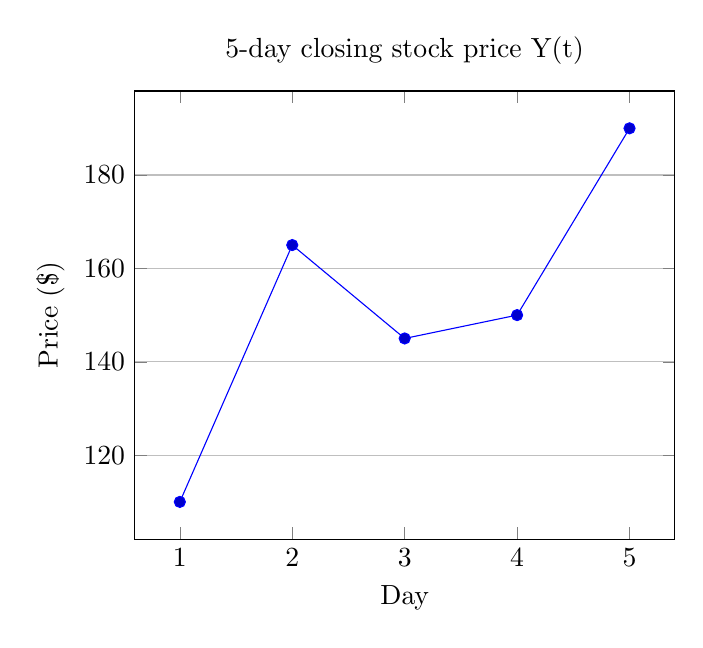
\begin{tikzpicture} 
		\begin{axis}[xlabel=Day,ylabel=Price (\$), ymajorgrids, title=5-day closing stock price Y(t)] 
			\addplot coordinates { 
				(1,110) 
				(2,165) 
				(3,145) 
				(4,150) 
				(5,190) 
			}; 
		\end{axis} 
	\end{tikzpicture}
\end{center}

Consider the the daily closing stock price for a company, $Y(t)(t=1,2,\ldots,5)$, such that $Y(1) = 110$, $Y(2) = 165$, $Y(3) = 145$, $Y(4) = 150$ and $Y(5) = 190$. The universe of discourse needs to cover the range of between the highest and lowest values you are considering, which in this case is $110$ and $190$. To aide explanation of the example the universe of discourse is set as the range $[100,200]$.

This example considers one linguistic variable which indicates the performance of a stock. The universe of discourse is partitioned into equal length intervals, $\left\{u_1, u_2,\ldots,u_k\right\}$, such that $u_1 = [100 \ldots 120]$, $u_2 = [120 \ldots 140]$, $u_3 = [140 \ldots 160]$, $u_4 = [160 \ldots 180]$ and $u_5 = [180 \ldots 200]$. Fuzzy sets are then defined which are the linguistic values of the linguistic variable ``Performance", $very\_low$, $low$, $mid$, $high$ and $very\_high$. These fuzzy sets consist of the grade of membership of each interval in the fuzzy set. For example:
\begin{description}
\item[] $very\_low = 1/u_1 + 0.5/u_2 + 0/u_3 + 0/u_4 + 0/u_5$
\item[] $low = 0.5/u_1 + 1/u_2 + 0.5/u_3 + 0/u_4 + 0/u_5$
\item[] $med = 0/u_1 + 0.5/u_2 + 1/u_3 + 0.5/u_4 + 0/u_5$
\item[] $high = 0/u_1 + 0/u_2 + 0.5/u_3 + 1/u_4 + 0.5/u_5$
\item[] $very\_high = 0/u_1 + 0/u_2 + 0/u_3 + 0.5/u_4 + 1/u_5$
\end{description}
where the symbol $+$ denotes the union operator. $F(t)$ the time series of these fuzzy sets, and can be regarded as a linguistic variable.

\Cref{def1} shows that $F(t)$, derived from $Y(t)$, is a fuzzy time series of the linguistic variable ``Performance'' with fuzzy sets $f_i(t) (i=1,2,\ldots)$ as its linguistic values. \Cref{def2} states that, for a first order fuzzy time series, there is a relationship $R$ between $F(t-1)$ and $F(t)$ for all time $t$ in the time series. This is called a fuzzy logical relationship and is denoted as $F(t-1) \rightarrow f(t)$.

Following from the example, $Y(t)$ is mapped to the fuzzy time series $F(t)$ where $F(1)=low$, $F(2)=high$, $F(3)=med$, $F(4)=med$ and $F(5)=very\_high$. The fuzzy logical relationships can be shown as follows: 

\begin{table}[h]
	\center
	\begin{tabular}{ l l l }
  	$low \rightarrow high$  \\
  	$high \rightarrow med$ \\
  	$med \rightarrow med$ \\
  	$med \rightarrow very\_high$ \\
	\end{tabular}
	\caption{Fuzzy Logical Relationships}
\end{table}

\Cref{def3} states fuzzy logical relationships that share the same left-hand side value may be grouped into fuzzy logical relationships groups. The fuzzy logical relationship groups for the example are as follows:

\begin{table}[h]
	\center
	\begin{tabular}{ c c c c }
  	Group 1: & $low$ & $\rightarrow$ & $high$ \\
  	Group 2: & $med$ & $\rightarrow$ & $med, very\_high$ \\
  	Group 3: & $high$ & $\rightarrow$ & $med$ \\
	\end{tabular}
	\caption{Fuzzy Logical Relationship Groups}
\end{table}

These relationships are then used to forecast observations in time. Taking $t+1$ as the point in time to be forecast, we forecast a fuzzy value $F(t+1)$ using the fuzzy logic relationship grouping where the left-hand side is $F(t)$. If there is no fuzzy logical relationship group for $F(t)$, then $F(t)$ is forecast.

The forecast value or values for $F(t+1)$ are defuzzified by taking the mean of the midpoints of the intervals which have a maximum membership in the forecast fuzzy sets. This crisp value forecast for $Y(t+1)$.

To illustrate, if $F(t)$ is $med$, then the fuzzy logical relationships group with a matching left-hand side is Group 2. From this the forecast fuzzy values for $F(t+1)$ are $med$ and $very\_high$. The maximum intervals for these fuzzy sets are $u_3$ and $u_5$ respectively. The midpoint of these intervals are $150$ for $u_3$ and $190$ for $u_5$, with a mean value $\frac{150 + 190}{2}=170$. This crisp value is used as the forecast.

\subsection{Higher-order Fuzzy Time Series}

\begin{ftsdef}
\label{def5}
Suppose $F(t)$ is caused by $F(t-1),F(t-2),\ldots,F(t-n)$ simultaneously, then the fuzzy logical relationship, $R$, for $F(t)$ can be represented by $F(t-n)\rightarrow F(t)$, $F(t-2) \rightarrow F(t)$, $\ldots$ and $F(t-1) \rightarrow F(t)$, then F(t) is a higher-order fuzzy time series and is denoted as an $n$th-order fuzzy time series.
\end{ftsdef}

\Cref{def5} defines a higher-order fuzzy time series. \cite{tsai1999study} developed a procedure which maintains the captures of higher-order time series while maintaining the simplicity of first-order calculations.

On an $m$-order fuzzy time series, $F(t)$ is caused by $F(t-1)$, $F(t-2)$, $\ldots$, and $F(t-m)$ simultaneously. The $m$ fuzzy logical relationships for $F(t)$ are obtained in the same manner as a first-order model. The relationships can be represented as follows:

\begin{table}[H]
	\center
	\begin{tabular}{ c }
  	$F(t-1) \rightarrow F(t)$ \\
  	$F(t-2) \rightarrow F(t)$ \\
  	\vdots \\
  	$F(t-m) \rightarrow F(t)$ \\
	\end{tabular}
	\caption{Higher-Order Fuzzy Logical Relationships}
\end{table}

The relational function for an expression $F(t-k) \rightarrow F(t)$ is shown as $R^{m}_{k}(t)$. In an $m$-order fuzzy time series for any forecast $F(t)$ there are $m$ relational functions $R^{m}_{\ \ 1}, R^{m}_{\ \ 2}, \ldots, R^{m}_{\ \ m}$, where $R^{m}_{\ \ k}=R(t,t-k)$. In $R^{m}_{\ \ k}$, the $m$ indicates what order model the relation is for the $i$ represents the first-order fuzzy relation between $F(t-k)$ and $F(k)$, for all $k={1,2,\ldots,m}$. For example, the relational matrix representing the fuzzy logical relationships between observations 2 points in time apart on a third-order fuzzy time series could be shown as:

\begin{table}[H]
	\center
	\begin{tabular}{ c }
  	$R^{3}_{\ \ 2}(1) = F(1) \times F(3)$ \\
  	$R^{3}_{\ \ 2}(2) = F(2) \times F(4)$ \\
  	\vdots \\
  	$R^{3}_{\ \ 2}(k) = F(k) \times F(k-2)$ \\
	\end{tabular}
	\caption{Second-Order Fuzzy Logical Relationships}
	\label{second-order-rels}
\end{table}

\Cref{second-order-rels} shows the equations for the second-order fuzzy logical relationships. For a third-order fuzzy time series, the fuzzy logical relationships for $R^{3}_{\ \ 1}(t)$ and $R^{3}_{\ \ 3}(t)$ will also need to be computed for all times $t$. Once these values are obtained, $R^{m}_{\ \ n}$ represents the set of $n$-order fuzzy logical relationship groups. The forecast values for $F(i)$ can be found from each fuzzy logical relationship group:

\begin{table}[H]
	\center
	\begin{tabular}{ c }
  	$F_{i1} = F_{i-1} \circ R^{m}_{\ \ 1}$ \\
  	$F_{i2} = F_{i-2} \circ R^{m}_{\ \ 2}$ \\
  	\vdots \\
  	$F_{im} = F_{i-m} \circ R^{m}_{\ \ m}$ \\
	\end{tabular}
	\caption{Forecast Values for $F(i)$}
\end{table}

Where $F_{ik}$ is the collection of fuzzy values forecast by the fuzzy logical relationship group $R^{m}_{\ \ k}$. Since the above relations happen simultaneously, the forecast for $F(i)$ is the intersection of all $F_{ik}$, which are the forecast fuzzy values common to each order of fuzzy logical relationship groups used . These values are then defuzzified as in \Cref{fts-design}.

\subsection{Ratio-based Interval Selection}

The following method for ratio-based interval selection was studied by \cite{huarng2006ratio}.

\begin{table}[H]
	\center
	\begin{tabularx}{0.5\textwidth}{ X R }
  	MIN$(r_1,\ldots,r_{n-1})$ & Base\\
  	\hline 
  	\noalign{\smallskip}
	$\leq 0.05\%$ & $0.01\%$ \\
	$\leq 0.5\%$ & $0.1\%$ \\
	$\leq 5.0\%$ & $1\%$ \\
	\ldots & \ldots
	\end{tabularx}
	\caption{Base Mapping Table for Ratios}
\end{table}

\begin{description}
\item[Step 1] Calculate the relative difference between adjacent observations such that $r_t=|x_t-x_{t-1}|/x_{t-1}$ for all $t$
\item[Step 2] Determine the $base$ by mapping MIN$(r_1,\ldots,r_{n-1})$ to the base mapping table
\item[Step 3] Plot the distribution for all $r_t$ according to the determined $base$
\item[Step 4] Choose a sample percentile $\alpha$, such as $\alpha=50\%$. Select a $ratio$ which is the smallest relative difference that is larger than $\alpha$
\item[Step 5] Calculate the intervals 

\begin{table}[H]
	\center
	\begin{tabular}{ c }
	  	$u_1 = [lower_1, upper_1]$ \\
	  	$u_2 = [lower_2, upper_2]$ \\
	  	\vdots \\
	\end{tabular}
\end{table}

The beginning of the first interval, $lower_1$, is set to MIN$(x_t)-c$ where MIN$(x_t)$ is the lowest observation and c is some small constant. The $interval\_length$ for the time series is set to $lower_1 \times ratio$. The upper bound of the first interval, $upper_1$, is set to $lower_1 + interval\_length$. The remaining intervals are calculated using the formula $[lower_k,upper_k]=[lower_{k-1}+interval\_length+c, upper_{k-1}+interval\_length+c]$ for all $k=(2,3,\ldots)$.
\end{description}

\subsection{Root Mean Squared Error}

%make random walk model heterosedastic, as in stock markets do not follow random walks

\section{Implementation}

\subsection{Framework Development}

\subsection{Fuzzy Logic Toolkit}

\subsection{Optimisation}

\subsubsection{Lazy-evaluation}

\subsubsection{Search optimisations}

\section{Results \& Evaluation}

\subsection{Comparison Models}

\section{Conclusion}

\section{Future work}

\appendix

\section{technical analysis Techniques}

\label{app:tatechniques}

There are many trading strategies that use technical analysis. Almost any strategy that uses past price movement or behaviour as an indicator for future price counts as a technical trading strategy. Discussed here are 3 techniques that are seen to be widely used in technical trading strategies.

\subsection{Trend Identification}
Moving averages are graph lines that indicate the average price over a fixed period. Different functions can also be used such as calculating a weighted moving average. Its purpose is to smooth the noise in a graph and to identify a trend. A moving average cross is where 2 moving averages are used on a graph, generally with one having a short period indicating current trend and one having a long period indicating overall trend. When the line of the short period crosses the line of the long period it is an indication of a change in trend \citep{brock1992}. Moving averages have been used in many studies on technical trading strategies, with generally positive performance. \cite{taprofitability} found moving average rules showed consistently profitable results in the foreign exchange and futures market, and the most reliable performance in the stock market out of the methods tested.

\subsection{Pattern Identification}
Technical Patterns are visual patterns that appear in a graph of price movement. A Head-and-Shoulders pattern is one where the price represents a persons head an shoulders, where the price shows an approximately symmetrical sequence of five local extrema which correspond to 2 shoulders, 2 necks and a head. The outcome of this pattern is that the price moves down. \cite{foundations} examined 10 of these patterns and found overwhelming significance for the indicators when applied to the Nasdaq stock index. \cite{chang1999methodical} also find a Head-and-Shoulders pattern was profitable, but was outperformed by simpler trading rules such as a moving average indicator. Japanese Candlestick charting is considered to be identifying technical patterns.

\subsection{Price Levels}

\begin{figure}[H]
    \centering
    \includegraphics[width=0.8\textwidth]{images/uptrend.png}
    \caption{Visual Support Line}
\end{figure}

Pivot points, Support and Resistance price levels which are very commonly calculated in industry but have not received significant academic attention \citep[p. 55]{osler2000support}. According to \cite{murphy1999technical}, a support level is ``a level or area on the chart under the market where buying interest is sufficiently strong to overcome selling pressure. As a result, a decline is halted and prices turn back up again''. Resistance is the opposite of support. Often they are levels where the price has had difficulty breaking before, either as static price points (such as the weekly low price) or points where the price meets a trend line that it appears to be bounding off. \cite{brock1992} found strong support for this style of trading strategy.


\bibliographystyle{apa}
\bibliography{dissertation}

\end{document}
